\subsection{Experimental  Evaluations}\label{sec:experiments}
In this section, we empirically evaluate the accuracy and performance of FACTS.  We perform two sets of experiments.  The first, measures the error in terms of number of complaints above or below the threshold as a function of the total number of complaints.  The second, measures the performance overhead for messaging and complaint as a function of the threshold.  


\subsubsection{Experimental parameters}
For our experiments, we set the maximum number of complaints per epoch $n=1,000,000$.  If we consider an epoch of one day, this results in approximately 11.6 complaints per second. To understand accuracy and efficiency of FACTS, we measure them for a range of thresholds $100 \le t \le 1000$.  With these fixed, we set the remaining parameters according to Corollary~\ref{cor:params}.  In particular, we set the server's storage $s=96n=12MB$.  The user set size $u$ varies from (approximately) 47,000 to 470,000 bits, while the message set size $v$ goes from (approximately) 740 to 7400.  

% \paragraph{Current total number of complaints (background complaints) $m$. } m is the counts of all complaints on the server in current epoch. For the complaints of any single message, $m$ also plays the role of background noise. The maximum number of background complaints will be less than 1 million per day if each complain takes 100ms on average. In the experiments one epoch is set to be one day and m is ranging from 100k to 1000k. 

% \paragraph{Table size $s$. } 
% $s$ shows the space usage for server to store the bit vector for active complaints for current epoch. The table size is preset by the server. Our goal is to keep s small for space efficiency but sufficiently large to handle the maximum number of complaints within one epoch, which is 1 million in our experiments. The table size is set to 96 million bits accordingly, which takes 12MB storage on server. % want it be small, MB. 86400s / 100ms ~ 1 million  % epoch could be longer, 1 day -> < 1 million

% \paragraph{Number of slots assigned to each user. } $u$ is preset by server in terms of the number of total messages per day and the desired explicit threshold. This is also the size of communication package size between server and users. To avoid slowing down the process, we want to keep the size of each communication smaller than 64k Bytes, which is the maximum size of one TCP package. In the experiments, we set the number of slots for user to: $u = 47.31 * n / t$.  n is the number of total complaints within one epoch and is bounded by 1 million as described above. % Why: This is the bottleneck, u should be small enough fit inside 64kB. 

% \paragraph{Number of slots assigned to each message. } $v$ is decided in terms of the desired explicit threshold: $v = 7.409 * t$. 

% \paragraph{Tipping point (Implicit threshold) $\tau$. }
% Recall the equation (3) in Section IV, the implicit threshold can be decided by given background complaints $m$, size of user set $u$, size of message $v$, table size $s$ and explicit threshold $t$. In accuracy experiments, to result of a list of expected explicit thresholds, which in our experiments we choose them from 100, 400, 700 and 1000, the implicit thresholds are calculated accordingly. 

% \paragraph{Setup for experiments. } For accuracy evaluation, simulations on all configurations with combination of our chosen $m$, $u$, $v$ and $t$, are running locally. Statistics are collected based on 1000 runs of each configuration. 

\begin{figure*}
\hspace*{-0.7in}
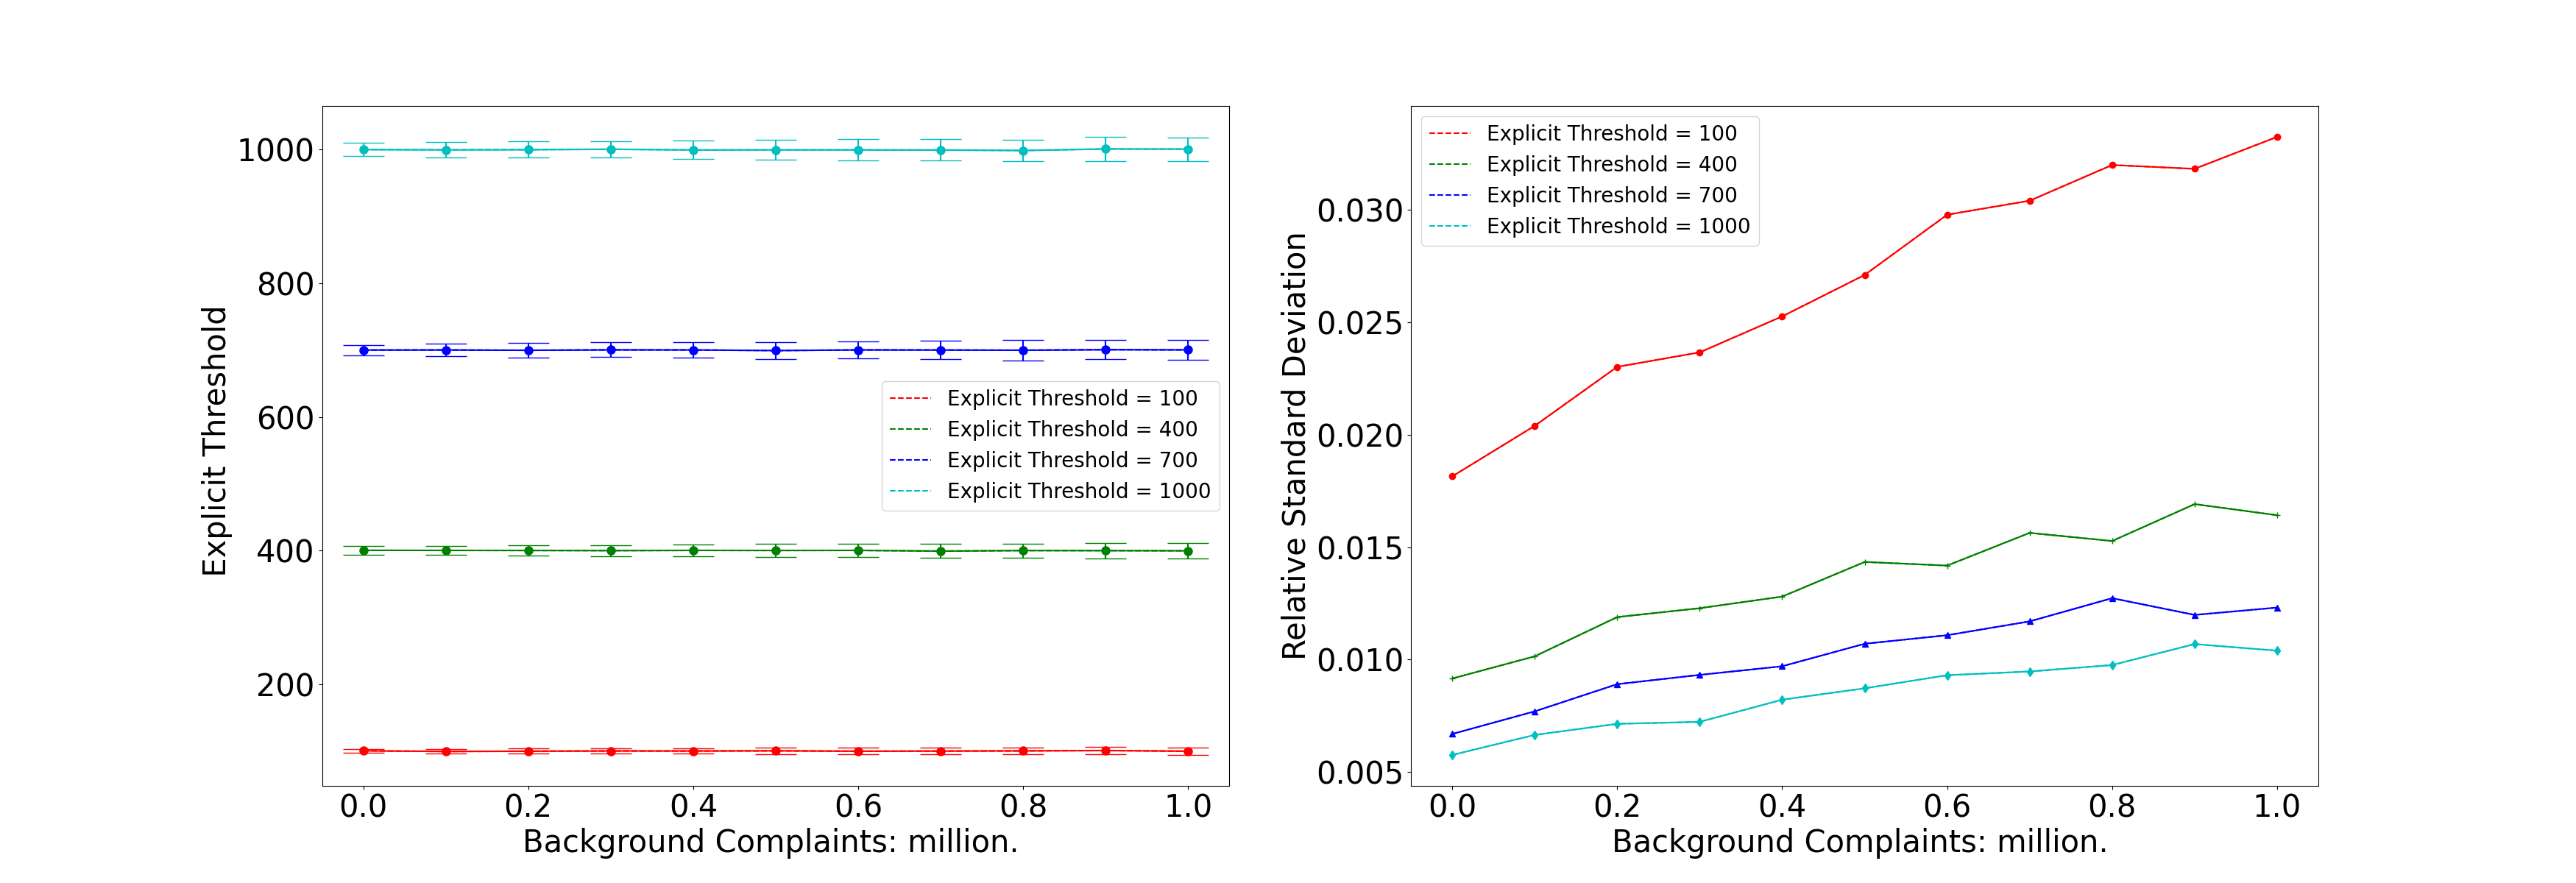
\includegraphics[width=1.2\textwidth]{src/facts/imgs/ExplicitThresholdPlotsTitleless.png}
\centering
\caption{The (left) Mean and (right) Relative Standard Deviation of Experimental Explicit Threshold vs. The Number of Background Complaints.}
\label{fig:Accuracy}
\end{figure*}

\begin{figure}
  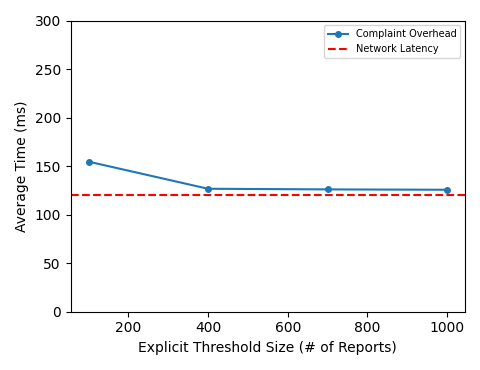
\includegraphics[width=\linewidth]{src/facts/imgs/var_threshold_size.png}
  \caption{Average complaint time as a function of the threshold with $n=1,000,000$ complaints per epoch.  Complaint time is measured as the average of 100 samples and has a variance of less than 5ms.  Network latency shows the minimum latency required to transmit 3 sequential messages over the network, a lower bound on complaint time.}
  \label{fig:report_msg_threshold}
\end{figure}

\subsubsection{Accuracy and stability} 
To measure the accuracy of FACTS, we observe the actual number of complaints necessary to cause an audit on a single message as a function of the background noise (i.e., total complaints on other messages).  We calculate both the mean and the standard deviation of this value to capture the accuracy and stability of the complaint mechanism.  To get a statistically meaningful estimate of these, our experiments run 1000 iterations of each parameter configuration.

The results of our experiments are presented in Figure~\ref{fig:Accuracy}.  The left side of this figure shows the mean number of complaints to trigger an audit for a given threshold $t$.  As can be seen from the error bars, the absolute errors in number of complaints is quite small, with a maximum deviation of about 10 complaints at a threshold of 1000.  Not surprisingly, we see that this error increases as the background noise increases, but the mean number of complaints remains remarkably steady at the desired value.  The right side of Figure~\ref{fig:Accuracy} shows the relative standard deviation of the number of complaints as a function of background noise.  From this graph we can see that the relative error is only a few percent, with a maximum relative error of about 3.5\%.  Not surprisingly, the threshold 100 measurement incurs the highest relative error because the noise is a much higher ratio when compared to the threshold.  These experiments suggest that FACTS achieves good accuracy for a wide variety of threshold and background noise.

% For accuracy experiments, in order to avoid the impact caused by randomness of the system, we perform a series of independent experiment on each configuration, simulating the behaviours among server and users. Each simulation is based on one configuration of parameters below in terms of an desired explicit threshold. The experimental explicit thresholds, which is the actual number of complaints take place to trigger an audit are collected. The ideal result for the experimental explicit thresholds should be exactly the desired explicit threshold with no fluctuation. By varying number of background complaints $m$ and adjusting other parameters, we are expecting a horizontal line of the experimental explicit thresholds for each desired explicit threshold. 
% What we measure and expect


% Figure~\ref{fig:Accuracy}. left shows the accuracy and stability of desired explicit threshold as a function of number of background complaints. Results are across over explicit thresholds 100, 400, 700 and 1000. With varying number of background complaints, our construction of FACTS consistently achieves the desired explicit thresholds. With 1000 runs on each point, the absolute errors are consistently low. The error rate is slightly increasing as the number of background complaints grows up, and reach the maximum with 1 million background complaints (equivalent to the number of total messages per epoch). The maximum deviation is around 10 over desired threshold 1000. The accuracy is still outstanding even with pushing the desired explicit threshold down to 100 as an extreme scenario. Each line suggests a robust accuracy FACTS achieves for different desired explicit threshold. 

% Furthermore, Figure~\ref{fig:Accuracy}. right shows the relative error rate of desired explicit threshold as a function of number of background complaints. With the desired explicit threshold being 100, the maximum relative error of is achieved, which is under 3.5\% with 1 million background complaints. The relative error for explicit threshold is decreasing while setting higher explicit thresholds. The results from simulations suggest our construction a probabilistic approach which achieves a deterministic explicit over certain degree, which in our experiment is 96%, with advanced guarantee of privacy and efficiency (next section). 

% \begin{figure}
%     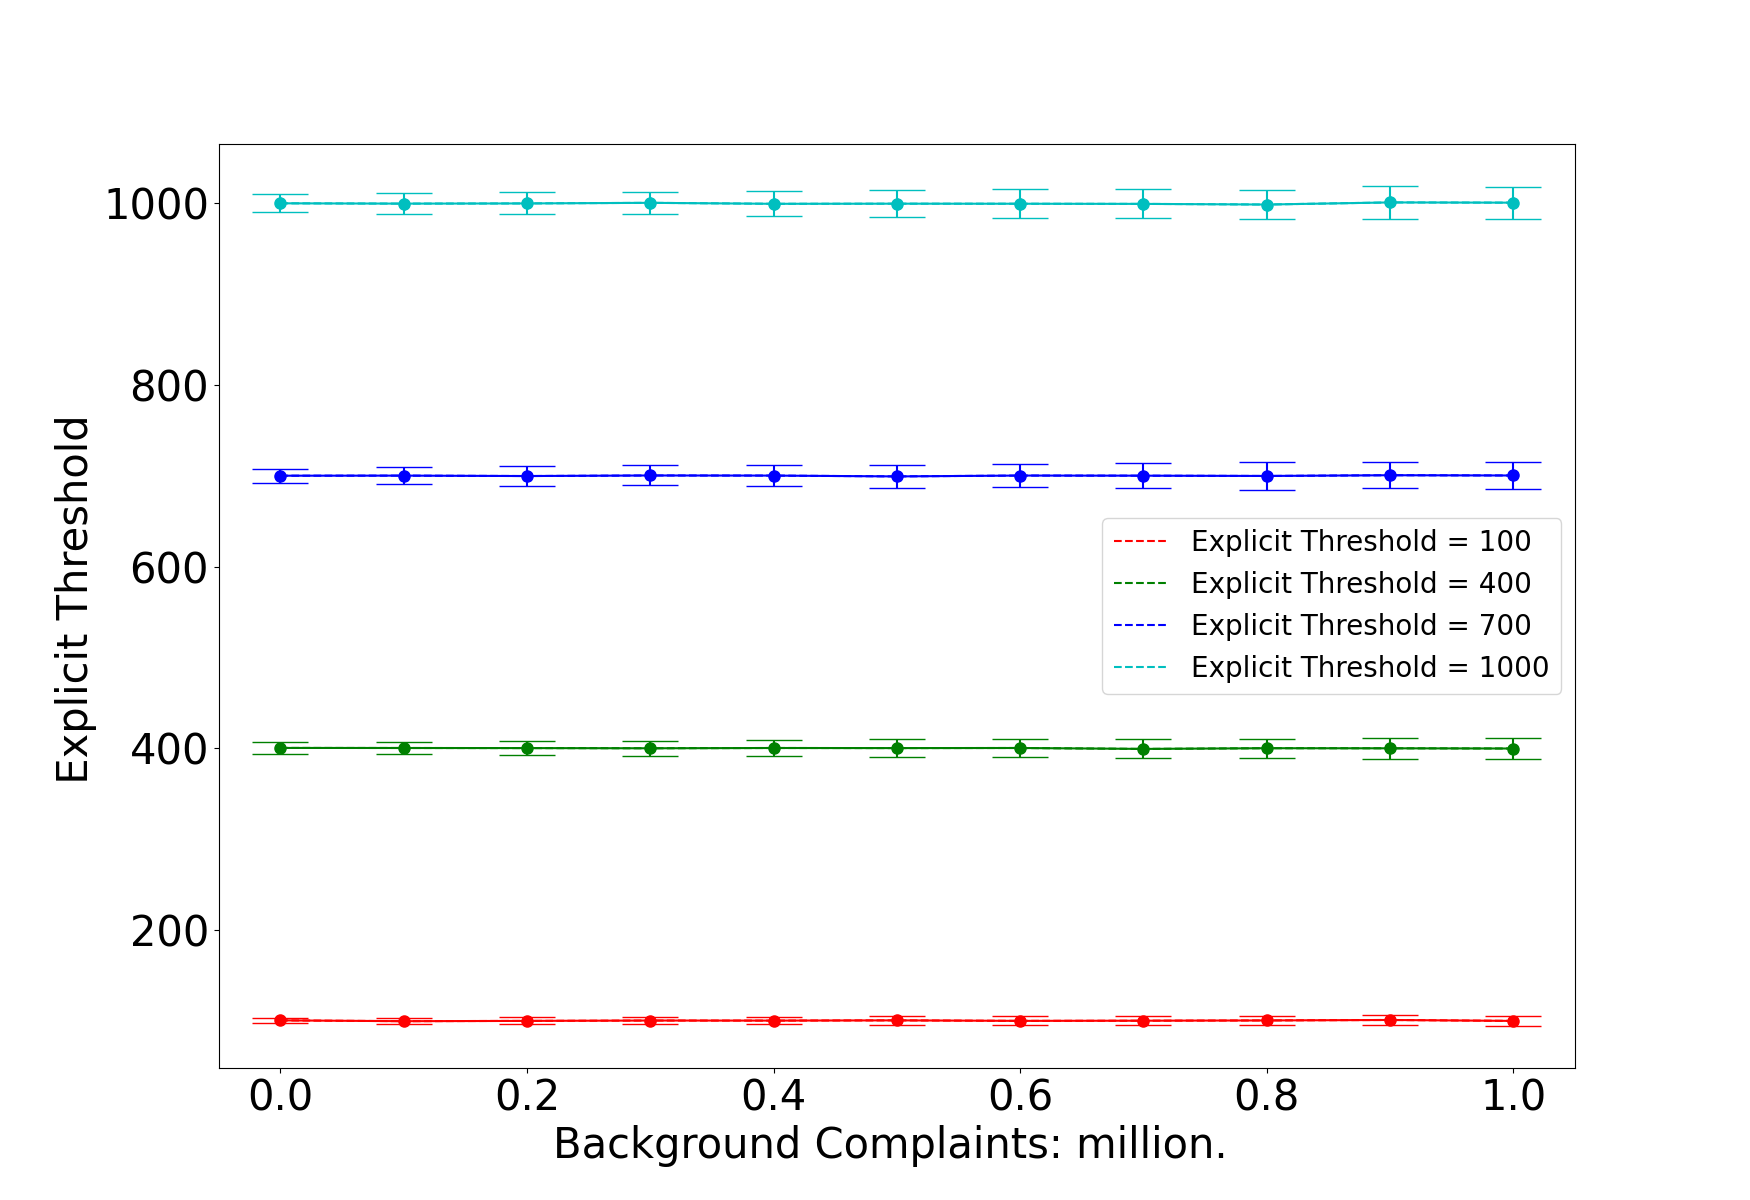
\includegraphics[width=0.5\textwidth]{imgs/MeanETTitleless.png}
%     \label{fig:Mean}
%     \caption{The Explicit Threshold vs. The background complaints. }
% \end{figure}


% \begin{figure}
%     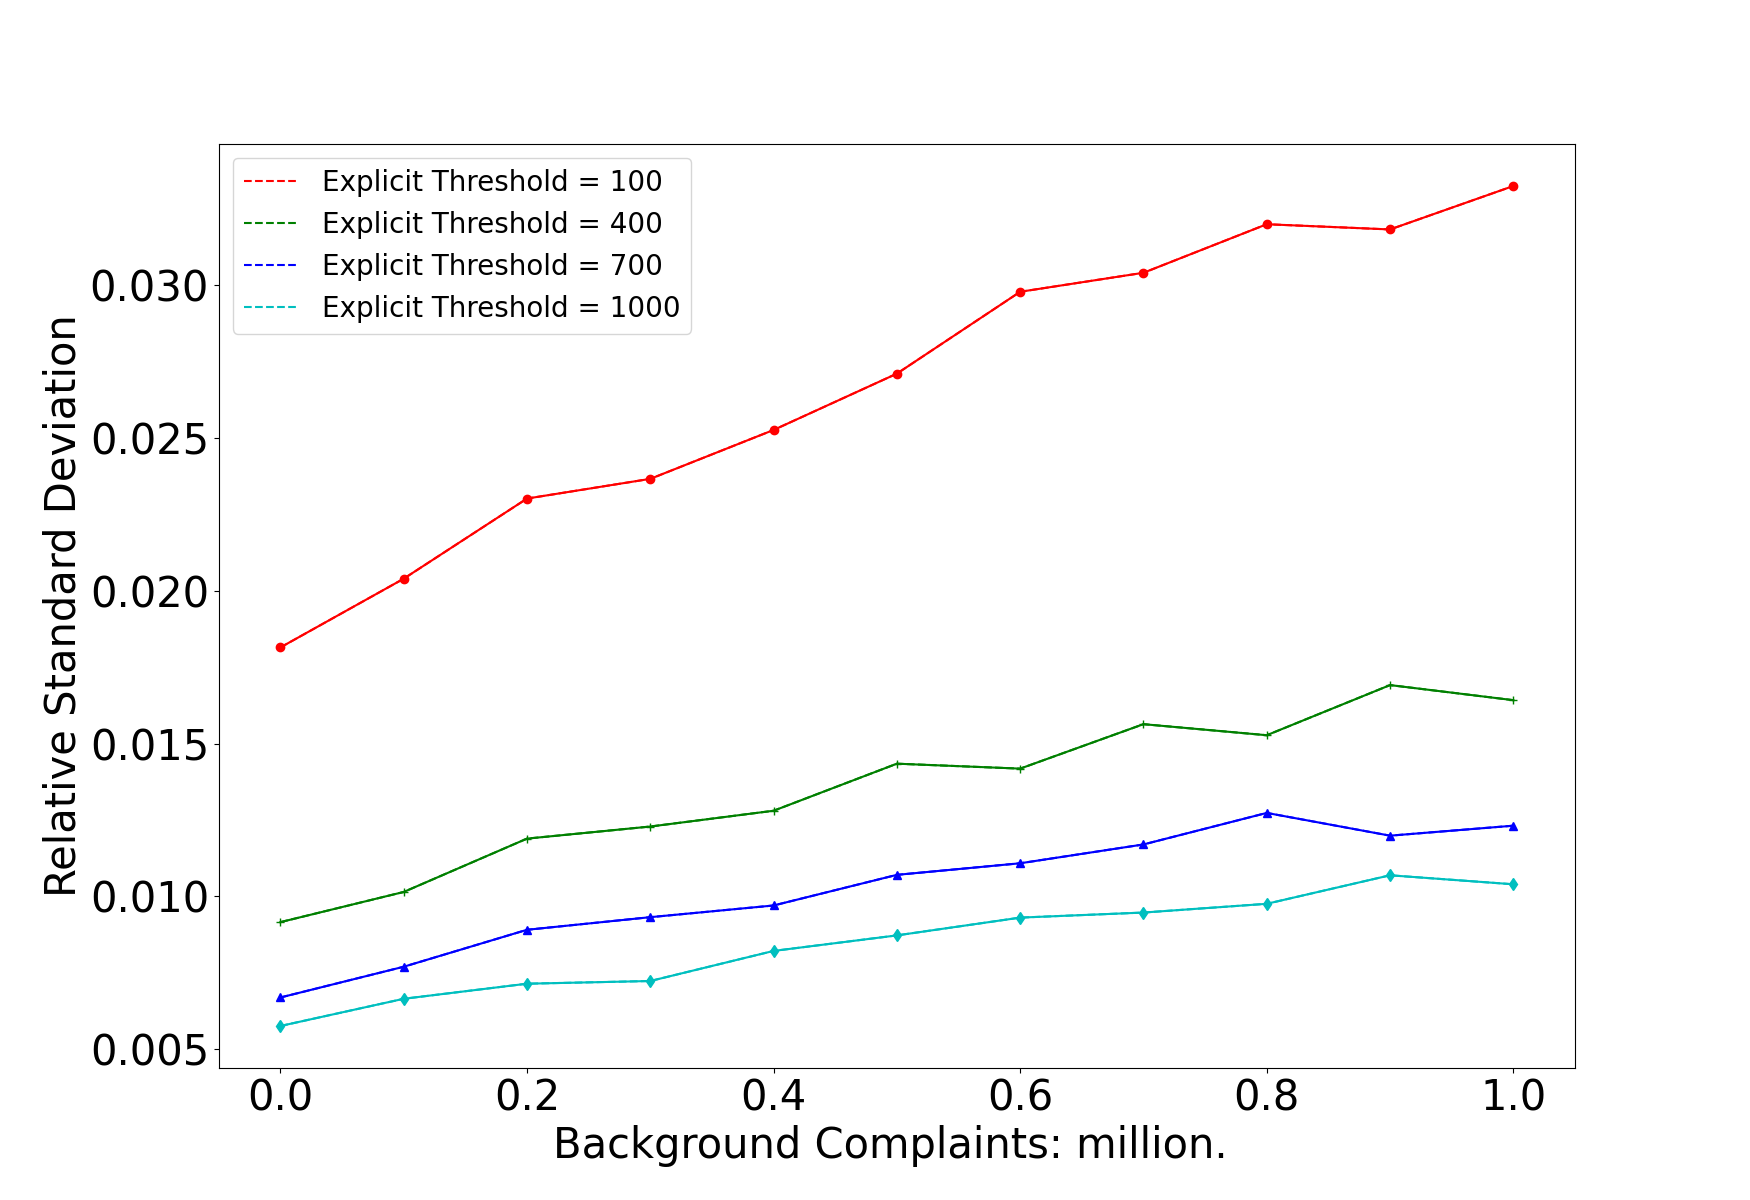
\includegraphics[width=0.5\textwidth]{imgs/RelativeSDETTitleless.png}
%     \caption{The Relative Standard Deviation of Explicit Threshold vs. The background complaints. }
%     \label{fig:SD}
% \end{figure}


% If inserting both figures together:

% \textbf{Replacing words used in plots and marked in the paragraph to the correct terminology}

% \alert{figure y should be relative errors on two different noise levels}

\subsubsection{Performance overhead}

Our next set of experiments measures the performance overhead of FACTS as a function of the threshold to start an audit.  Specifically, we measure the overhead of sending a message using FACTS, and the cost of issuing a complaint.  We note that for the message sending cost, we do not measure the cost of the EEMS communication, instead only measuring the added overhead due to FACTS.

For these experiments, we implemented both the client and server using the Rust programming language.  We used SHA-3 for a hash function, and for encryption and signatures we used Rust's ring library\cite{ring} implementation of OpenSSL's ChaCha20-Poly1305 protocol and Ed25519 respectively. To instantiate the CCBF, we used a simple library bitvec\cite{bitvec} that allows memory to be bit addressed, rather than byte addressed, which gains us a quick, compact way to store the CCBF data structure. 

To simulate network overhead, we implemented a simple web server and client, which communicated over a (simulated) 8 Mbps network with a latency of 80ms, using TLS 1.3.  Since we are only measuring the overheads of FACTS over the underlying EEMS, our measurements 
did not include the time to send the message over the EEMS, nor the time to establish the TLS connection. All experiments were run on a 4.7Ghz Intel Core i7 with 16GB of RAM, with a sample size of 100 for each metric.  As in the accuracy experiments, we set $n=1,000,000$ and threshold varying from 100 to 1000, with the remaining parameters determined by Corollary~\ref{cor:params}.

For our measurement of message origination we looked at the cost of originating and sending a message of size 2MB. Creating and sending such a message with the encrypted hash and identity took 98ms, which indicates that the major bottleneck in this process is the 80ms network latency. We see then that when a user wishes to forward a message, they will still call $\orig(A,x)$, but then forward the original message whereas in an EEMS this would just require a forward.  Thus, the overhead of FACTS on a forward is slightly less than 100ms.

Figure~\ref{fig:report_msg_threshold} shows our measurements of the time to issue a complaint as a function of the audit threshold.  The time for this is dominated by the time to retrieve the user set (i.e., the bits that the user can write) from the server.  Since the size of this set $u=O(n/t)$, this time grows inversely with the threshold $t$.  Thus, as the threshold increases, the total complaint time decreases very quickly, going down to essentially just the network latency when $t\ge 400$.

These experiments show that both the (added) cost of sending messages and the cost of complaints (for sufficiently large $t$) are dominated by the networking costs.  Thus, as long as the latency of the network is reasonable, FACTS can scale to millions of complaints per day.